\documentclass[letterpaper]{article}
\usepackage[submission]{aaai2027}
\usepackage[hyphens]{url}
\usepackage{graphicx}
\urlstyle{rm}
\def\UrlFont{\rm}
\usepackage{natbib}
\usepackage{caption}
\usepackage{placeins}
\frenchspacing
\usepackage{amsmath,amssymb}
\usepackage{booktabs}
\definecolor{samblue}{RGB}{0,114,178}
\definecolor{medorange}{RGB}{230,159,0}
\definecolor{wsigreen}{RGB}{0,158,115}
\definecolor{fewred}{RGB}{213,94,0}
\pdfinfo{/TemplateVersion (2027.1)}
\setcounter{secnumdepth}{2}

\title{FewClick: A Few-Click Interactive Framework for User-Specified Histopathological Tissue Segmentation}
\author{Anonymous Submission}
\affiliations{}

\begin{document}
\maketitle

\begin{abstract}
Tissue segmentation in whole-slide images (WSIs) underpins tissue quantification, tumor-microenvironment analysis, and computer-assisted pathology. Existing supervised methods, however, typically require predefined tissue classes and extensive pixel-level annotations, limiting their ability to accommodate task-specific tissue definitions. General-purpose promptable segmentation models accept interactions such as points and boxes, but rely primarily on local visual appearance. Without explicit representations of cellular composition, tissue hierarchy, and long-range slide context, they struggle to identify spatially disconnected yet semantically consistent tissue from a few local prompts. We introduce FewClick, a cell-aware hierarchical region prompting framework for few-prompt binary segmentation of a user-specified tissue against the remainder of a WSI. FewClick constructs boundary-adaptive multiscale region tokens, enriches them with cell embeddings, density, and composition, and propagates sparse hierarchical context. A signed set encoder represents positive and negative prompts, while a region decoder predicts the target across the slide and projects region probabilities to pixels. With one positive and one negative point, FewClick achieves 0.7418 macro Dice on matched patch episodes, outperforming SAM by 0.2769. On 5 WSIs and 12 tissues, its outcome-blind macro Dice is $0.5659\pm0.0700$, a 41.4\% relative gain over WSI-SAM despite an oracle localization advantage given to the baseline.
\end{abstract}

\section{Introduction}
Whole-slide images (WSIs) capture complete tissue morphology at gigapixel resolution and support tumor measurement, tumor-microenvironment analysis, region-of-interest selection, and downstream diagnostic modeling. Their complex boundaries and substantial scale variation, however, make dense pixel-level annotation expensive. Existing tissue segmenters usually predict predefined label spaces \cite{chan2019histosegnet,xu2019camel,tokunaga2019awmf,vanrijthoven2021hooknet}; study-specific structures or new tissue definitions therefore require additional annotations and retraining.

Promptable methods such as RITM, SimpleClick, and the Segment Anything Model (SAM) instead specify a target from sparse points, boxes, or scribbles \cite{sofiiuk2022ritm,liu2023simpleclick,kirillov2023sam}. Their direct application to WSIs nevertheless faces three challenges. First, tissue identity depends not only on color and texture but also on cell types, density, and spatial composition \cite{graham2019hovernet,horst2024cellvit}. Second, the same tissue may occur in multiple disconnected regions, so a local prompt must convey semantics beyond its immediate neighborhood. Third, pathology spans cell morphology, local architecture, and global layout, while a single scale rarely preserves both precise boundaries and reliable tissue identity. These difficulties are compounded by gigapixel inference and prompt selection \cite{deng2023sam_pathology,liu2024wsisam}.

Prompted WSI segmentation should therefore infer the tissue concept intended by a few interactions and retrieve semantically consistent regions across the slide rather than only expand a local boundary around each click. Our key observation is that visually similar regions may differ in cellular composition, whereas disconnected instances of the same tissue can share cellular and architectural patterns. This motivates a region-level representation that combines visual boundaries, cellular evidence, and hierarchical context.

Figure~\ref{fig:overview} summarizes FewClick. Aligned multiscale features form learnable tissue regions that are enriched through cell-to-region attention and connected by a sparse parent--child hierarchy. Separate set encoders aggregate positive and negative prompts into a target representation, and a context-aware decoder predicts all fine regions before projecting their probabilities back to pixels.

Our contributions are fourfold. (1) We formulate WSI segmentation as prompt-defined binary tissue retrieval rather than fixed-channel multiclass prediction. (2) We introduce differentiable, cell-aware tissue regions that jointly encode visual features, cell embeddings, density, and composition. (3) We design sparse bottom-up and top-down interaction across aligned fine, intermediate, and coarse regions. (4) We combine signed prompt encoding with context-aware region decoding to use positive and negative evidence throughout the slide. Controlled comparisons show consistent gains over three promptable baselines, while ablations verify the contributions of learnable regions, cellular evidence, and multiscale context.

\section{Related Work}
\subsection{Tissue Segmentation in Whole-Slide Images}
Most WSI tissue models use fixed label spaces. HistoSegNet and CAMEL learn segmentation from weak labels \cite{chan2019histosegnet,xu2019camel}, as do slide-level MIL and CLAM for classification \cite{campanella2019clinical,lu2021clam}. AWMF-CNN, HookNet, and DMMN exploit multiscale context \cite{tokunaga2019awmf,vanrijthoven2021hooknet,ho2021dmmn}, while CTransPath and UNI pretrain transferable pathology encoders \cite{wang2022ctranspath,chen2024uni}. None uses sparse prompts to define a new tissue mask at inference.

\subsection{Promptable Pathology Segmentation}
RITM and SimpleClick refine object masks from clicks \cite{sofiiuk2022ritm,liu2023simpleclick}, while SAM generalizes promptable mask prediction \cite{kirillov2023sam}. MedSAM and SAM-Med2D adapt this paradigm to medical data \cite{ma2024medsam,cheng2023sammed2d}. Pathology evaluations expose challenges from dense instances, gigapixel scale, and prompt selection \cite{deng2023sam_pathology}, whereas WSI-SAM couples two resolutions for breast-lesion segmentation \cite{liu2024wsisam}. These methods mainly delineate a prompted object; FewClick retrieves semantically consistent, potentially disconnected tissue.

\subsection{Cell-Aware Hierarchical Modeling}
HoVer-Net and CellViT encode nuclear morphology \cite{graham2019hovernet,horst2024cellvit}, whereas ST-Net and HE2RNA link H\&E to gene expression \cite{he2020stnet,schmauch2020he2rna}. OCELOT uses tissue context for cell detection \cite{ryu2023ocelot}; Ceograph, HACT-Net, and Patch-GCN model cell or patch relations \cite{wang2023ceograph,pati2022hact,chen2021patchgcn}; and HIPT aggregates cellular, tissue, and slide-level information \cite{chen2022hipt}. They target nuclei, cells, or slide-level prediction rather than prompt-defined region masks.

\section{Method}
\begin{figure*}[!t]
\centering
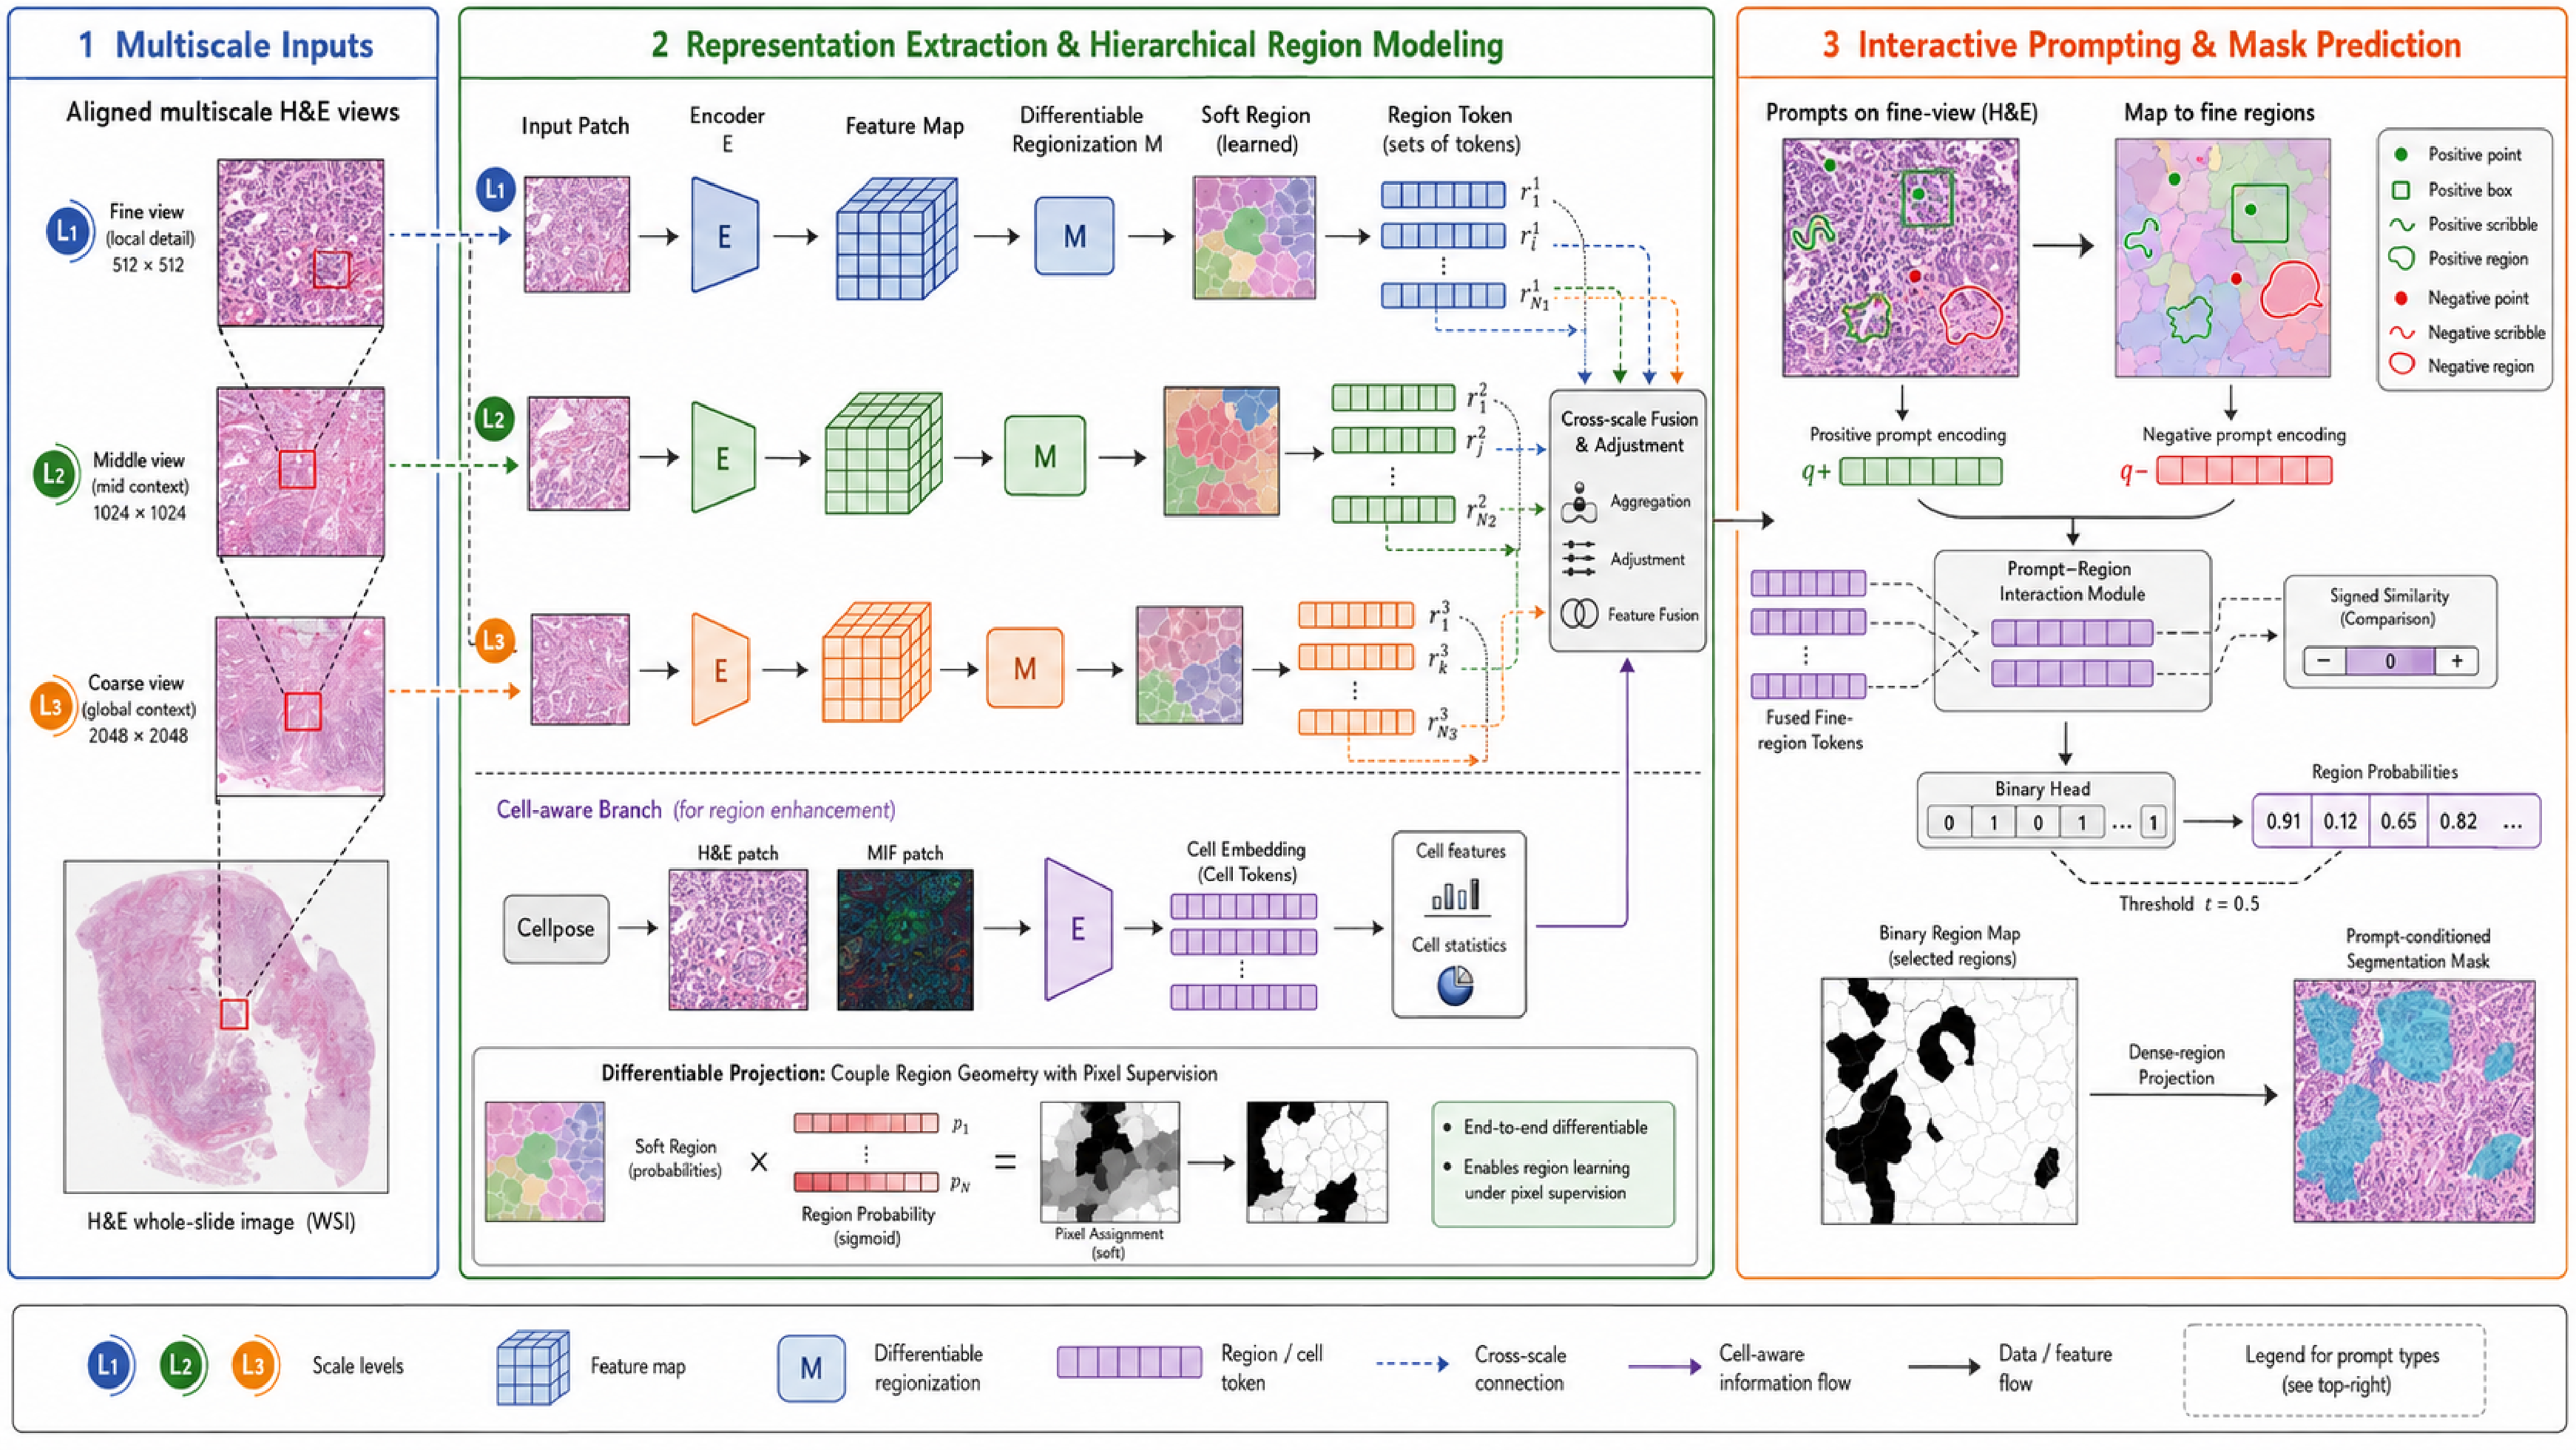
\includegraphics[width=\textwidth]{images/main_picture.pdf}
\caption{Overview of FewClick. Aligned multiscale features are partitioned into learnable regions, fused with cell evidence, and propagated through a sparse hierarchy. Positive and negative prompts define the target tissue; a context-aware decoder predicts fine-region probabilities, which are projected to pixels as the final mask.}
\label{fig:overview}
\end{figure*}

FewClick formulates interactive WSI segmentation as tissue retrieval from a few signed prompts. A user marks a local example of the target tissue and a confusable non-target region; the model then identifies all regions with consistent cellular composition and tissue semantics, including target areas disconnected from the prompts. Rather than perform dense global reasoning over pixels, FewClick converts aligned multiscale images into learnable tissue regions, enriches them with cellular evidence, propagates context across scales, and decodes every region under the current prompt-defined task. This region-level formulation preserves fine boundaries, cellular cues, and large-scale organization while keeping WSI inference sparse.

Figure~\ref{fig:overview} summarizes the pipeline. Multiscale encoders extract aligned fine, intermediate, and coarse features, from which assignment heads form differentiable regions and visual tokens. A separately pretrained cell encoder supplies morphology, density, and composition through cell-to-region attention. A sparse parent--child graph then exchanges local and macroscopic context. Given positive and negative prompts, set encoders construct a task representation, and a graph decoder combines prompt evidence, spatial neighborhoods, and hierarchical context to predict target probabilities. Soft region assignments finally project these probabilities back to pixels.

\subsection{Prompt-Defined Tissue Segmentation}
Conventional semantic segmentation binds output channels to tissue classes fixed during training. FewClick instead treats each interaction as target-versus-rest segmentation: positive prompts specify what to retrieve, whereas negative prompts specify what to exclude. The same model can therefore segment different tissue concepts without changing a class-specific output head.

Let $I$ be an H\&E-stained WSI and $\Omega$ its reference-resolution pixel domain. Given positive and negative prompt sets $\mathcal{P}^{+}$ and $\mathcal{P}^{-}$, FewClick learns
\begin{equation}
f_{\theta}(I,\mathcal{P}^{+},\mathcal{P}^{-})=\widehat{M},\qquad
\widehat{M}\in[0,1]^{|\Omega|}.
\label{eq:problem}
\end{equation}
where $\widehat{M}(x)$ is the target probability at $x\in\Omega$. Episodes vary the target tissue and prompt configuration, forcing $f_\theta$ to infer each task from local evidence rather than memorize a class--channel mapping.

\subsection{Molecularly Guided Cell Learning}
Tissue identity depends not only on color and texture but also on cellular morphology, phenotype, density, and composition. FewClick therefore uses an independent cell branch to provide microscopic evidence. This branch describes cells without directly determining tissue borders, preventing a few atypical cells from dominating region formation.

For detected cell $i$, let $u_i$ be its center in reference coordinates. The cell representation combines normalized position, log cell area, a one-hot nuclei-class label, and an XCellFormer embedding extracted from an H\&E neighborhood centered at $u_i$:
\begin{equation}
z_i=[u_i,\log(1+a_i),h_i,e_i],\qquad
z_i\in\mathbb{R}^{D_z},\quad i=1,\ldots,N,
\label{eq:cell}
\end{equation}
where $a_i$ is cell area, $h_i$ is the nuclei-class one-hot vector, $e_i$ is the learned cellular embedding, $N$ is the cell count, and $D_z$ is the resulting dimension. XCellFormer is pretrained on registered H\&E and multiplex immunofluorescence data using molecular expression supervision. Its extracted features are used to supply cell-level morphology and phenotype information.

The resulting pairs $\{(u_i,z_i)\}_{i=1}^{N}$ associate microscopic evidence with learned regions after morphology-based region formation.

\subsection{Multiscale Adaptive Regionization}
Cell morphology, local architecture, and global tissue layout require different fields of view. FewClick extracts three physically aligned scales and compresses each dense feature map into a small set of learnable regions. Unlike fixed superpixels, these regions receive gradients from the final prompted segmentation objective and can adapt their boundaries to the downstream task.

\paragraph{Spatially aligned multiscale features.}
We extract views with a shared center and progressively larger physical fields of view,
\begin{equation}
\{I_s\}_{s\in\mathcal{S}},\qquad \mathcal{S}=\{f,m,c\},
\label{eq:scales}
\end{equation}
where $f$, $m$, and $c$ denote fine, intermediate, and coarse scales. A scale-specific encoder maps each view to
\begin{equation}
F_s=E_s(I_s),\qquad F_s\in\mathbb{R}^{H_s\times W_s\times D},
\label{eq:features}
\end{equation}
where $H_s\times W_s$ and $D$ denote the feature-grid size and visual dimension. All $F_s$ share a physical coordinate system.

\paragraph{Differentiable soft region assignment.}
At scale $s$, an assignment head predicts logit $a_s(x,k)$ for feature-grid position $x\in\Omega_s$ and region $k\in\{1,\ldots,K_s\}$. The normalized membership is
\begin{equation}
A_s(x,k)=\frac{\exp a_s(x,k)}{\sum_{j=1}^{K_s}\exp a_s(x,j)},
\qquad \sum_{k=1}^{K_s}A_s(x,k)=1,
\label{eq:assignment}
\end{equation}
and the initial visual token is
\begin{equation}
r_{s,k}=
\frac{\sum_{x\in\Omega_s}A_s(x,k)F_s(x)}
{\sum_{x\in\Omega_s}A_s(x,k)+\varepsilon},
\qquad r_{s,k}\in\mathbb{R}^{D}.
\label{eq:pool}
\end{equation}
Here, $K_s$ is the region count and $\varepsilon>0$ ensures numerical stability. Because $A_s$ is used for both pooling and pixel projection, segmentation errors directly refine region boundaries.

\paragraph{Region pretraining.}
To prevent fragmented or collapsed assignments, we pretrain the region encoder with SLIC \cite{achanta2012slic} as a weak prior. Following differentiable superpixel learning \cite{jampani2018ssn}, boundary, compactness, balance, and purity losses stabilize assignments without fixing the final partition.

\subsection{Cell-Aware Region Modeling}
Visual tokens alone may confuse tissues with similar appearance but different cellular composition. FewClick softly associates cells with each region and lets the region query the most informative ones. Spatial membership restricts where evidence originates, whereas content attention determines which cells best characterize the region.

Let $\xi_s(u_i)$ map $u_i$ to the scale-$s$ feature grid, with $A_s(\xi_s(u_i),k)$ bilinearly interpolated. For the $N_s$ visible cells, content affinity is
\begin{equation}
e_{s,k,i}=
\frac{(W_qr_{s,k})^{\top}(W_kz_i)}{\sqrt{D_a}},
\label{eq:cell-affinity}
\end{equation}
where $D_a$ is the attention dimension. Spatially weighted attention is
\begin{equation}
\alpha_{s,k,i}=
\frac{A_s(\xi_s(u_i),k)\exp(e_{s,k,i})}
{\sum_{j=1}^{N_s}A_s(\xi_s(u_j),k)\exp(e_{s,k,j})+\varepsilon}.
\label{eq:cell-attention}
\end{equation}
The cellular context is
\begin{equation}
c_{s,k}=\sum_{i=1}^{N_s}\alpha_{s,k,i}W_vz_i,
\qquad c_{s,k}\in\mathbb{R}^{D},
\label{eq:cell-context}
\end{equation}
In addition to attention pooling, we explicitly retain a soft-assignment-calibrated cell-count statistic. Let $\bar A_{s,k,i}=A_s(\xi_s(u_i),k)/\sum_{\ell=1}^{K_s}A_s(\xi_s(u_i),\ell)$ and let $\gamma_s=N_s^{\mathrm{total}}/\max(\lvert\mathcal{I}_s\rvert,1)$ correct for the retained cells in the feature cache. We compute
\begin{equation}
\rho_{s,k}=\log\!\left(1+\gamma_s\sum_{i\in\mathcal{I}_s}\bar A_{s,k,i}\right),
\label{eq:cell-count}
\end{equation}
where $\mathcal{I}_s$ indexes retained valid cells. Thus, $\rho_{s,k}$ is the log of the estimated cell count assigned to region $k$, rather than an area-normalized physical density. Nuclei-class composition, cell area, spatial location, and embedding-distribution information are represented implicitly by the attention-pooled context $c_{s,k}$ instead of by separate hand-crafted proportion or moment features. The cell-aware token is
\begin{equation}
\widetilde r_{s,k}=
\operatorname{MLP}\!\left(
\operatorname{LN}[r_{s,k},c_{s,k},\rho_{s,k}]
\right).
\label{eq:cell-fusion}
\end{equation}
The explicit count preserves low cellularity as evidence for adipose, mucinous, or necrotic tissue.

\subsection{Sparse Hierarchical Reasoning}
One scale cannot simultaneously provide precise boundaries and reliable tissue identity, yet dense attention over all WSI regions is intractable. FewClick instead constructs a sparse hierarchy from physical overlap: fine regions connect to covering intermediate regions, which connect to coarse regions. Bottom-up propagation lets macroscopic regions absorb local boundaries and cellular composition; top-down propagation returns broader tissue context to fine regions.

Let $\mathcal{V}_s$ be the scale-$s$ nodes and $\mathcal{C}(v)$ the children of parent $v$. We initialize
\begin{equation}
h_v^{(0)}=\widetilde r_v.
\label{eq:hier-init}
\end{equation}
For each intermediate or coarse parent, bottom-up aggregation is
\begin{equation}
\begin{split}
m_v^{\uparrow}
&=\operatorname{Attn}\!\left(
h_v^{(0)},\{h_u^{\uparrow}:u\in\mathcal{C}(v)\}
\right),\\
h_v^{\uparrow}&=h_v^{(0)}+m_v^{\uparrow}.
\end{split}
\label{eq:bottom-up}
\end{equation}
Fine nodes use $h_u^{\uparrow}=h_u^{(0)}$; intermediate nodes are updated before coarse nodes.

Let $\pi(k)$ and $\pi^2(k)$ be the parent and ancestor of fine region $k$. The updated upper-level context returns to that region through
\begin{equation}
h_{f,k}=h_{f,k}^{\uparrow}
+\tanh(\gamma)\operatorname{HAttn}\!\left(
h_{f,k}^{\uparrow},
[h_{\pi(k)}^{\uparrow},h_{\pi^2(k)}^{\uparrow}]
\right),
\label{eq:hierarchy}
\end{equation}
The learned scalar $\gamma$ starts at zero, making the adapter an identity map at initialization.

\subsection{Signed Prompt-Set Modeling}
Prompt count, type, and coverage vary across interactions, and one local example may represent only part of a tissue's appearance. FewClick therefore treats prompts as signed sets rather than an ordered sequence or a single averaged prototype. Positive prompts summarize shared target attributes, negative prompts describe confusable tissue to exclude, and their contrast defines the current task.

Soft assignments convert each prompt into a weighted combination of covered region tokens. Let
\begin{equation}
R^{+}=\{t_{\ell}^{+}\}_{\ell=1}^{n_+},\qquad
R^{-}=\{t_{\ell}^{-}\}_{\ell=1}^{n_-}
\label{eq:prompt-sets}
\end{equation}
be the positive and negative token sets. Permutation-invariant encoders \cite{zaheer2017deepsets,lee2019settransformer} produce
\begin{equation}
q^+=\operatorname{SetEnc}^{+}(R^+),\qquad
q^-=\operatorname{SetEnc}^{-}(R^-).
\label{eq:prompt-encode}
\end{equation}
The task token is
\begin{equation}
q=\operatorname{MLP}\left([q^+,q^-,q^+-q^-]\right).
\label{eq:task-token}
\end{equation}
The explicit difference contrasts target and exclusion evidence while each set encoder retains within-set diversity.

For node $v$, let $h_v$ denote Eq.~\eqref{eq:hierarchy} for fine nodes and $h_v^{\uparrow}$ otherwise. We combine prompt attention with prototype similarity:
\begin{equation}
\begin{split}
h_v^{\mathrm{prm}}
&=\operatorname{CrossAttn}\!\left(h_v,[R^+;R^-]\right),\\
s_v^+&=\cos(h_v,q^+),\qquad s_v^-=\cos(h_v,q^-).
\end{split}
\label{eq:prompt-match}
\end{equation}
Cross-attention uses distinct polarity embeddings. Its decoder input is
\begin{equation}
u_v=[h_v,q,h_v^{\mathrm{prm}},s_v^+-s_v^-,g_v],
\label{eq:node-feature}
\end{equation}
where $g_v$ encodes area, centroid, shape, scale, and relative position. Prompt associations and region targets are recomputed as assignments evolve.

\subsection{Context-Aware Mask Recovery}
Tissue regions are not independent: spatial neighbors exhibit local continuity, whereas cross-scale parent--child pairs share tissue semantics. FewClick jointly decodes these relations on a sparse region graph, so each prediction uses its own representation, prompt match, neighborhood, and hierarchical context. Soft projection then restores pixel probabilities without top-$K$ selection or class-specific area heuristics.

Let $\mathcal{G}=(\mathcal{V},\mathcal{E})$ contain all regions, same-scale spatial edges, and cross-scale parent--child edges. A sparse graph Transformer updates
\begin{equation}
\{\bar u_v\}_{v\in\mathcal{V}}
=\operatorname{GraphTr}\!\left(
\{u_v\}_{v\in\mathcal{V}},\mathcal{G}
\right).
\label{eq:graph-decode}
\end{equation}
For fine region $k$, the binary head gives
\begin{equation}
o_k=w_o^\top\bar u_{f,k}+b_o,\qquad p_k=\sigma(o_k),
\label{eq:region-prob}
\end{equation}
Fine-scale assignments project the probabilities to pixels:
\begin{equation}
\widehat M(x)=\sum_{k=1}^{K_f}A_f(x,k)p_k,\qquad x\in\Omega.
\label{eq:projection}
\end{equation}
We register $A_f$ to $\Omega$ before projection. This differentiable mapping avoids hand-crafted top-$K$, area, or threshold-selection heuristics; inference uses a fixed $0.5$ threshold. For a positive--negative conflict within one hard region, the system requests a finer prompt or higher-resolution interaction.

\subsection{Progressive Optimization and Inference}
The modules require supervision at different granularities, and optimizing all of them from random initialization can entangle region assignment, cell aggregation, and prompt decoding. We therefore train from local representations to the global task: cell and region encoders are stabilized first, cross-scale interaction is learned next, and prompt-conditioned segmentation is introduced last. This order follows the inference data flow while retaining region regularization during joint fine-tuning.

\paragraph{Progressive optimization.}
Training proceeds through cell pretraining, weakly guided region learning, cell-aware hierarchical learning, and episodic prompt-conditioned segmentation. Joint fine-tuning retains region regularization and uses reduced learning rates for pretrained encoders.

Episodes randomize prompt count, type, and coverage; hard negatives include adjacent tissue, feature-space neighbors, and high-confidence false positives.

The joint objective is
\begin{align}
\mathcal{L}={}&\mathcal{L}_{\mathrm{BCE}}
+\lambda_{\mathrm{D}}\mathcal{L}_{\mathrm{Dice}}
+\lambda_{\mathrm{B}}\mathcal{L}_{\mathrm{bd}}
+\lambda_{\mathrm{R}}\mathcal{L}_{\mathrm{reg}} \notag\\
&+\lambda_{\mathrm{A}}\mathcal{L}_{\mathrm{assign}}
+\lambda_{\mathrm{T}}\mathcal{L}_{\mathrm{task}}.
\label{eq:loss}
\end{align}
The first two terms supervise pixels, and $\mathcal{L}_{\mathrm{bd}}$ supervises boundaries. The soft target for $\mathcal{L}_{\mathrm{reg}}$ is
\begin{equation}
y_{f,k}=
\frac{\sum_{x\in\Omega_f}A_f(x,k)Y_f(x)}
{\sum_{x\in\Omega_f}A_f(x,k)+\varepsilon}.
\label{eq:region-target}
\end{equation}
Thus, $\mathcal{L}_{\mathrm{reg}}$ aligns $p_k$ with $Y_f$. $\mathcal{L}_{\mathrm{assign}}$ regularizes balance, entropy, compactness, and boundary consistency; $\mathcal{L}_{\mathrm{task}}$ separates positive target evidence from negative and non-target evidence.

\paragraph{Whole-slide inference.}
FewClick precomputes image features, cell embeddings, regions, and their hierarchy once per WSI. Each interaction updates only prompt encoding and region decoding before projecting fine-region probabilities to the mask. Decoding all regions, rather than growing from a clicked component, enables retrieval of distant and disconnected target tissue.

\section{Experiments}
% Do not allow later experiment floats to jump above this section heading on
% the partially filled preceding page.
\suppressfloats[t]\suppressfloats[b]
% Keep the two principal quantitative tables at the top of the experiments
% page. The qualitative results remain separate, numbered figures.
\begin{table*}[!t]
\centering
\begin{minipage}[t]{0.485\textwidth}
\vspace{0pt}
\centering
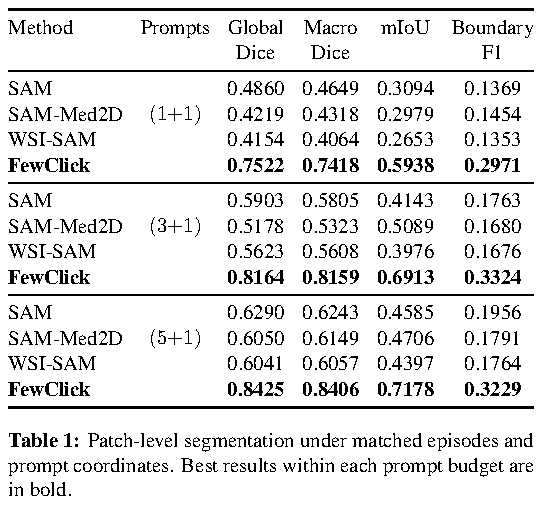
\includegraphics[width=\linewidth]{images/table_patch_comparison.pdf}
\refstepcounter{table}\label{tab:patch-comparison}
\end{minipage}\hfill
\begin{minipage}[t]{0.485\textwidth}
\vspace{0pt}
\centering
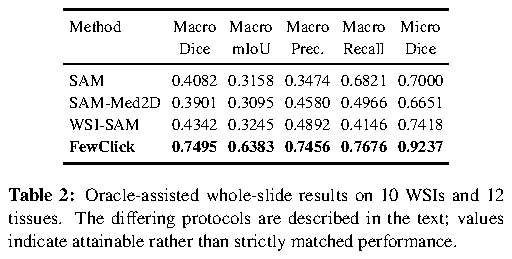
\includegraphics[width=\linewidth]{images/table_wsi_comparison.pdf}
\refstepcounter{table}\label{tab:wsi-comparison}
\vspace{3pt}

\raggedright\footnotesize
\textit{Whole-slide protocol.}
We evaluate 60 WSI--tissue tasks (5 WSIs $\times$ 12 tissues).
FewClick uses one positive and one negative point per task.
Five prompt sets are frozen before inference and summarized as an
outcome-blind mean$\pm$SD; one prompt-conflict abstention is scored
as empty. To favor the local baselines, GT identifies every positive
patch and supplies positive and negative points before the patch
predictions are stitched.
\end{minipage}

\end{table*}

\begin{figure*}[!t]
\centering
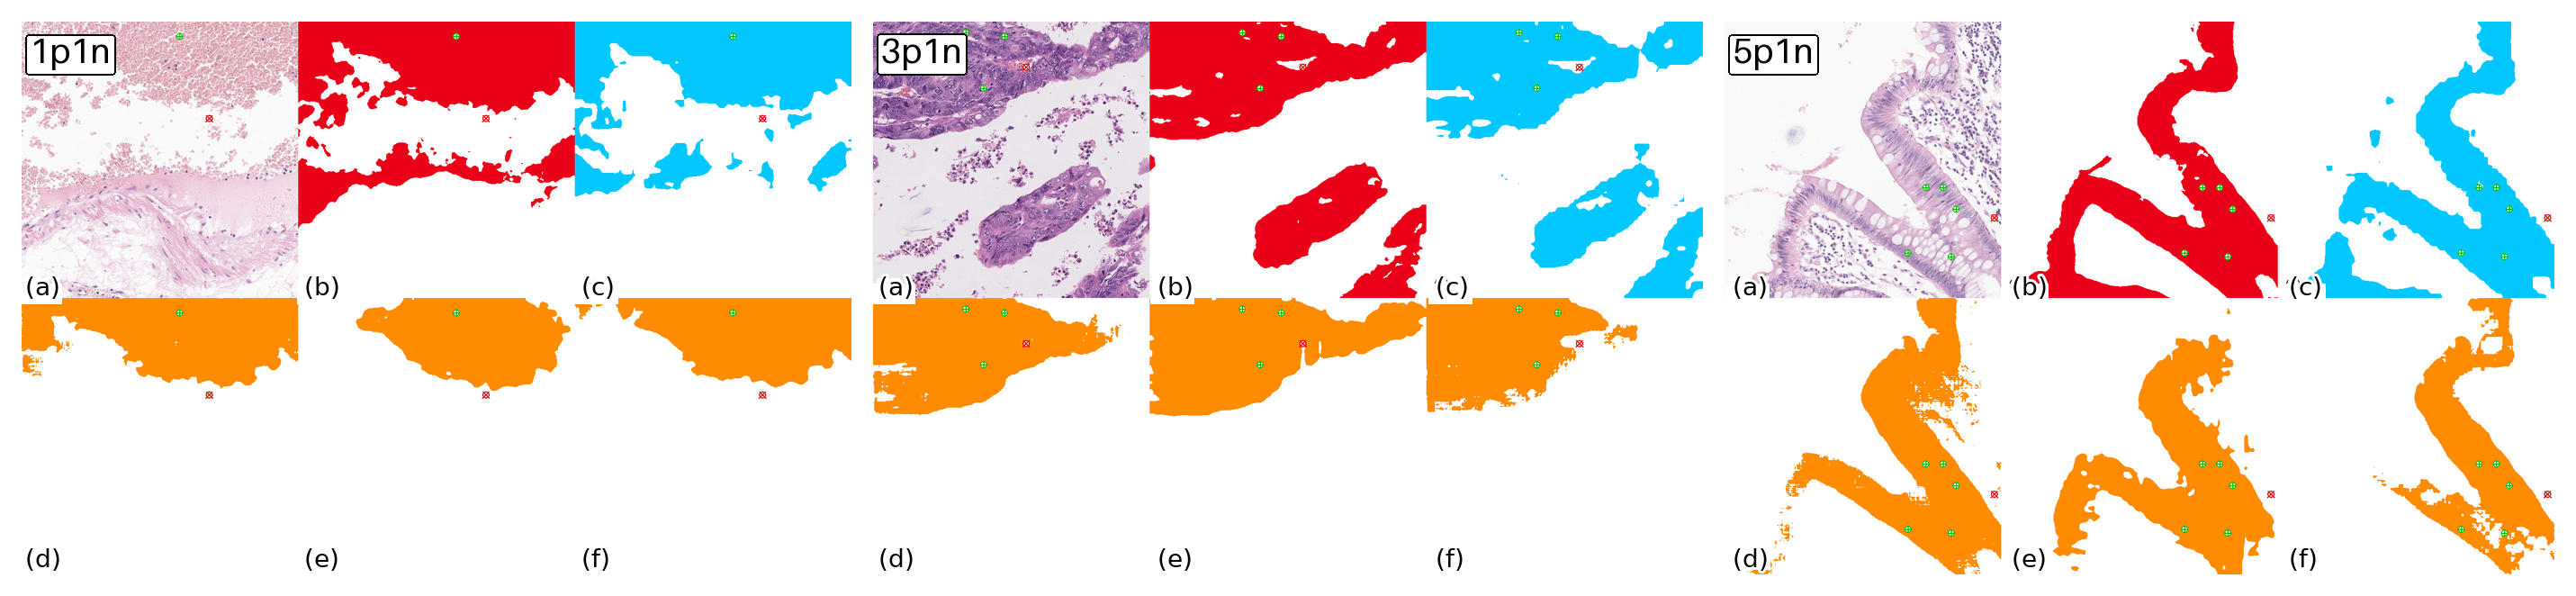
\includegraphics[width=\textwidth]{images/choosed/1p_3p_5p_horizontal_large_labels.png}
\caption{Patch-level qualitative examples under the $(1{+}1)$, $(3{+}1)$, and $(5{+}1)$ prompt budgets. In each group, (b) is the ground-truth (GT) mask, (c) is our prediction, and (d--f) are the predictions of three different SAM-based methods. Green and red markers denote positive and negative prompts, respectively.}
\label{fig:patch-qualitative}
\end{figure*}

\begin{figure*}[!t]
\centering
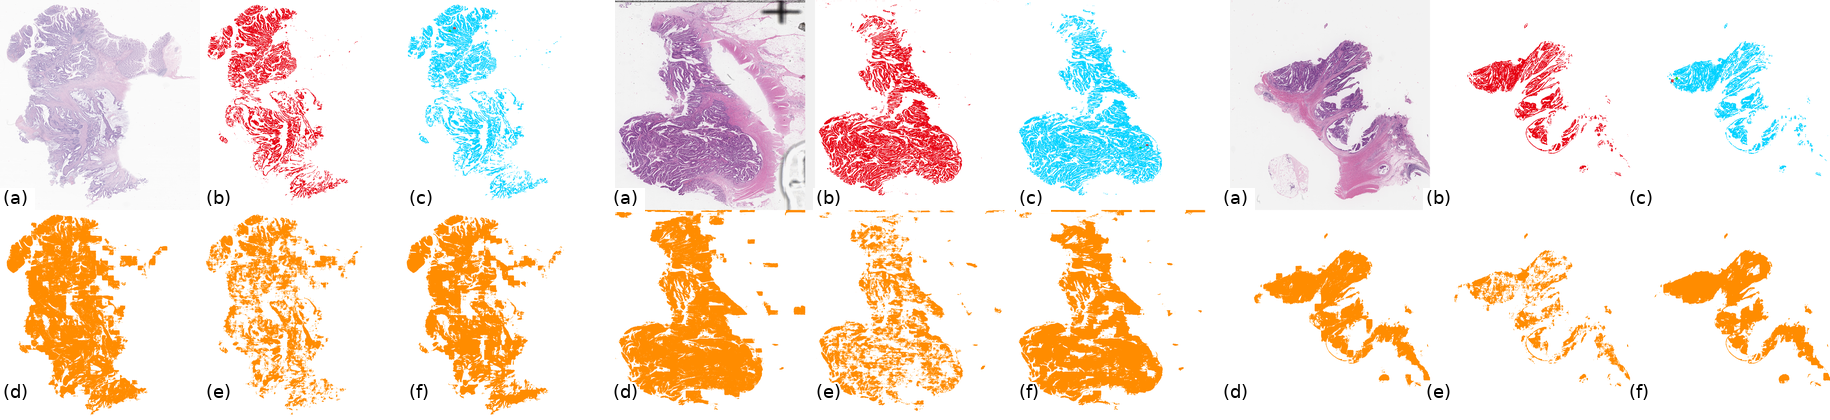
\includegraphics[width=\textwidth]{images/choosed/WSI_3panel_horizontal_matched_labels.png}
\caption{Whole-slide qualitative examples across three representative WSIs. In each group, (b) is GT, (c) is FewClick, and (d--f) are SAM-based predictions. FewClick uses one positive--negative prompt pair, whereas the baselines receive GT-guided patchwise prompts. The displayed FewClick masks are GT-selected best-of-five examples and illustrate attainable retrieval rather than the outcome-blind quantitative result.}
\label{fig:wsi-qualitative}
\end{figure*}

% Defer this one-column table until the preceding double-column float has
% shipped out; the opposite column can then be filled by the running text.

\subsection{Experimental Setup}
\paragraph{Data splits and episodic evaluation.}
We use a development cohort of 200 H\&E WSIs, split at the slide level into 140 training, 30 validation, and 30 held-out test slides. The test set remains sealed during model development. Ablations are conducted on a fixed validation manifest of 4,000 episodes; each training epoch contains 20,000 episodes. An episode specifies a WSI region, a target tissue, its binary mask, positive prompts, and optional hard negative prompts. Unless stated otherwise, all variants share the data split, prompt manifest, random seed, augmentation, and optimization schedule. Components downstream of an ablated representation are retrained to avoid distribution mismatch with the full-model decoder.

\paragraph{Baselines and metrics.}
We compare FewClick with SAM, SAM-Med2D, and WSI-SAM using their public pretrained weights without adaptation to our cohort. Patch-level methods receive identical images and prompt coordinates at each prompt budget. We report macro Dice (the primary metric), micro Dice, mIoU, and Boundary F1 with a two-pixel tolerance. Macro metrics weight episodes or tissue classes equally, whereas micro Dice aggregates pixel counts.

\subsection{Comparison with SOTA Models}
\paragraph{Patch-level results.}
We evaluate three interaction budgets, denoted $(1{+}1)$, $(3{+}1)$, and $(5{+}1)$ for one, three, or five positive points plus one negative point. FewClick leads every baseline under every budget and metric. With only $(1{+}1)$ prompts, it reaches 0.7522 global Dice and 0.7418 macro Dice, exceeding the strongest external baseline, SAM, by 0.2662 and 0.2769, respectively. Performance increases further with additional positive points, reaching 0.8425 global Dice under the $(5{+}1)$ budget.


Table~\ref{tab:patch-comparison} summarizes the matched-episode results. Because eligibility differs across budgets, we separately control for sample composition on their common subset: 885 occurrences from 819 unique patches, with identical masks, classes, and negative points. All four methods improve as the positive-point budget grows. FewClick rises from 0.7915 global Dice with one positive point to 0.8291 with three and 0.8425 with five. Thus, its advantage is not an artifact of changing episode composition, and additional positive evidence yields consistent gains on the controlled cohort (Figures~\ref{fig:patch-qualitative} and \ref{fig:prompt-budget}).



\paragraph{Whole-slide results.}
FewClick obtains $0.5659\pm0.0700$ macro Dice, exceeding WSI-SAM by 0.1658 (41.4\% relative); macro mIoU and micro Dice improve by 0.1895 and 0.0848, respectively (Table~\ref{tab:wsi-comparison}). Its lowest repeat (0.4557 macro Dice) remains above WSI-SAM (0.4001), showing that the average advantage is not driven by one favorable prompt set. SAM and WSI-SAM attain high recall but low precision despite oracle patch localization, whereas FewClick is more balanced. In a single deployment-style repeat, the 60 FewClick tasks use 120 points and 60 task-level WSI queries; each baseline uses 45,783 oracle-generated points and 23,642 local calls. These counts characterize interaction granularity rather than network forward passes or manual annotation time. FewClick outperforms the strongest SAM baseline in 11 of 12 tissues, with tumor epithelium as the exception (Table~\ref{tab:wsi-per-class}). Selecting the best of the same five candidates using GT raises macro Dice to 0.7493; we report this value only as an oracle sensitivity upper bound.

\begin{figure}[!t]
\centering
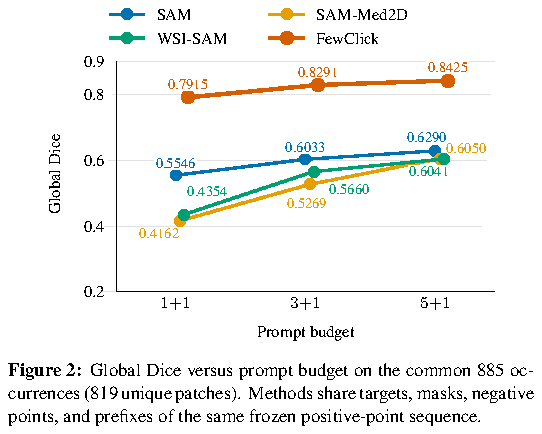
\includegraphics[width=\columnwidth]{images/figure_prompt_budget_curve.pdf}
\refstepcounter{figure}\label{fig:prompt-budget}
\end{figure}

\begin{table}[!t]
\centering
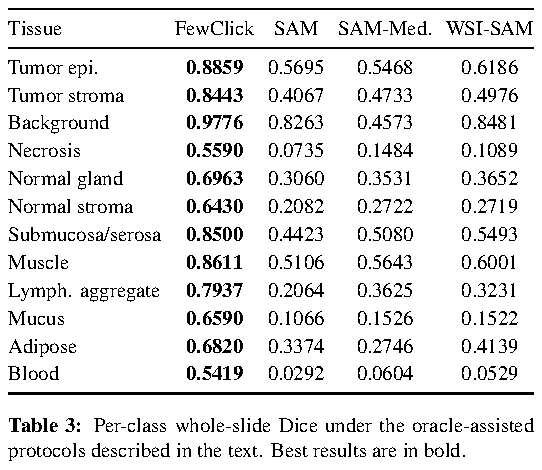
\includegraphics[width=\columnwidth]{images/table_wsi_per_class.pdf}
\refstepcounter{table}\label{tab:wsi-per-class}
\end{table}

\subsection{Ablation Studies}
We evaluate four architectural ablations on a fixed 4,000-episode validation set (Table~\ref{tab:ablations}); the sealed test split is not used. Removing or simplifying any component reduces performance.

\begin{table}[!t]
\centering
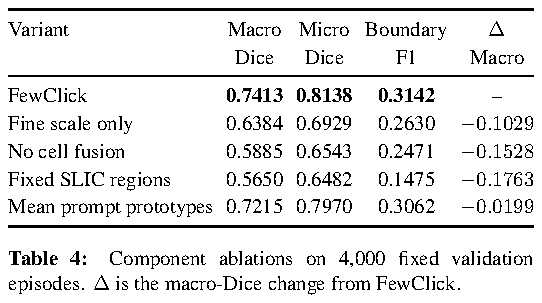
\includegraphics[width=\columnwidth]{images/table_ablation.pdf}
\refstepcounter{table}\label{tab:ablations}
% Locally tighten the gap before the following running text.

\end{table}

\paragraph{Learnable regions.}
Replacing differentiable assignment with 64 capacity-matched SLIC regions causes the largest degradation, reducing macro Dice by 0.1763 and Boundary F1 by 0.1667. The prompt-conflict rate also reaches 0.5645, showing that adaptive regions improve both spatial support and prompt--region alignment.

\paragraph{Cellular evidence.}
Removing cell-to-region attention, density, and cell statistics reduces macro Dice by 0.1528 and micro Dice by 0.1595, but Boundary F1 by only 0.0671. Cellular evidence therefore contributes mainly to tissue discrimination rather than boundary localization.

\paragraph{Multiscale context.}
Restricting FewClick to fine-scale regions reduces macro Dice by 0.1029 and micro Dice by 0.1209, versus 0.0512 for Boundary F1. Multiscale interaction thus primarily supports tissue identity and global retrieval while preserving local contours.

\paragraph{Prompt-set aggregation.}
Replacing the signed set encoder with masked positive and negative mean prototypes lowers macro Dice, micro Dice, and Boundary F1 under identical downstream training. Learned permutation-invariant aggregation therefore captures prompt-set structure beyond simple mean prototypes.

\subsection{Additional Experiment}
\paragraph{Cross-dataset generalization to an unseen tissue concept.}
We further test a tissue concept absent from training on an independent dataset excluded from model development. With all parameters frozen and tertiary lymphoid structures specified only through spatial prompts, FewClick achieves approximately $0.70$ Dice. Because this experiment covers one unseen concept with local prompt examples, we interpret it as few-shot cross-dataset generalization rather than fully open-world segmentation. Detailed data, prompt protocols, quantitative results, and qualitative examples are provided in the supplementary material.

\FloatBarrier

\section{Conclusion}
We studied the segmentation of user-specified tissue in whole-slide images (WSIs) from sparse interactive prompts and introduced FewClick. The method constructs learnable, boundary-adaptive tissue regions from physically aligned fine-, intermediate-, and coarse-scale fields of view. It injects microscopic evidence, including cell embeddings, cell density, and cell composition, into region representations through cell--region attention, and integrates local boundaries with global tissue context through sparse cross-scale hierarchical modeling. Positive and negative prompts are separately encoded as sets to define the tissue concept for the current task. A context-aware graph decoder then matches and predicts regions across the slide, while soft region assignments recover pixel-level masks. This design enables the model to retrieve spatially disconnected target regions that remain consistent in cellular composition and tissue semantics, rather than merely expanding connected areas around clicked locations.

Experiments show that, with one positive and one negative prompt on matched patch interaction episodes, FewClick improves macro Dice over SAM by 0.2769; this advantage persists under larger prompt budgets. Component ablations further demonstrate the complementary contributions of learnable regionization, cell-aware representations, multiscale hierarchical context, and set-based prompt encoding. These results indicate that incorporating microscopic cellular evidence and multiscale tissue structure into prompt-conditioned, region-level reasoning helps recover global tissue semantics from sparse local interactions.

Current cross-dataset validation remains limited in cancer types, staining conditions, and centers; broader multicenter evaluation is needed to establish robustness to domain shift. Performance also depends on prompt placement and coverage of tissue heterogeneity, so ambiguous or atypical clicks may provide insufficient evidence.

Future work will investigate domain-generalized training and evaluation across datasets and cancer types, combining multicenter data, domain-robust representations, and adaptation mechanisms for unseen tissue concepts to improve transferability in real pathology workflows. We will also explore strategies to reduce sensitivity to prompt placement, including uncertainty-based click recommendation, interactive prompt-quality assessment, prompt training robust to positional perturbations, and adaptive follow-up queries for conflicting or low-confidence predictions. These directions aim to obtain reliable whole-slide tissue segmentation with fewer and more stable interactions.

\bibliography{FewClick_AAAI27}
\end{document}
